% The two networks of a DeepONet: the branch reads the input
% function at the sensors, the trunk reads the point x, and the output is the
% sum of the products of their outputs.
\documentclass[tikz,border=2pt]{standalone}
% Shared preamble for the standalone TikZ figures of the talks.
%
% Every figure is a standalone .tex file in this folder, compiled to PDF with
% LuaLaTeX and included with \includegraphics at natural size, so its fonts
% match the slides (kpfonts-otf, as in the theme).
\usepackage{amsmath}
\usepackage{mathtools}
\usepackage{kpfonts-otf}
\usepackage{xcolor}
\usepackage{derivative}
\usepackage{tikz}
\usetikzlibrary{positioning,fit,arrows.meta,calc}

% Symbols used by the figures
\newcommand{\bm}[1]{\symbfit{#1}}
\newcommand{\Real}{\mathbb{R}}
\newcommand{\W}{\bm{w}}

% Node fills
\definecolor{nodeInput}{HTML}{EDEDED}
\definecolor{nodeOp}{HTML}{FBF6DE}
\definecolor{nodeOutput}{HTML}{E7F0FA}
\definecolor{nodeLayer}{HTML}{F1F1F1}
\definecolor{nodeGate}{HTML}{FBE9E7}
\definecolor{nodeState}{HTML}{E7F0FA}
\definecolor{backArrow}{HTML}{B03A2E}

\tikzset{
  edge/.style={-{Stealth[length=2.1mm]}, semithick},
  % computational graphs
  graphnode/.style={rectangle, draw=black!65, semithick, rounded corners=1.5pt,
    minimum height=8mm, minimum width=19mm, inner sep=3pt, align=center},
  inputnode/.style={graphnode, fill=nodeInput},
  opnode/.style={graphnode, fill=nodeOp},
  outputnode/.style={graphnode, fill=nodeOutput},
  % layer diagrams
  layernode/.style={graphnode, fill=nodeLayer, minimum width=13mm,
    minimum height=7.5mm},
  lossnode/.style={graphnode, fill=nodeOutput, minimum width=11mm,
    minimum height=7.5mm},
  backedge/.style={-{Stealth[length=2.1mm]}, semithick, draw=backArrow},
  elabel/.style={font=\footnotesize, inner sep=1.5pt},
  blabel/.style={font=\footnotesize, inner sep=1.5pt, text=backArrow},
  % recurrent cells
  gatenode/.style={rectangle, draw=black!65, semithick, rounded corners=1.5pt,
    fill=nodeGate, minimum height=7mm, minimum width=8mm, inner sep=2pt,
    font=\footnotesize},
  opcircle/.style={circle, draw=black!65, semithick, fill=white,
    inner sep=0pt, minimum size=5.2mm, font=\small},
  statenode/.style={graphnode, fill=nodeState, minimum width=11mm,
    minimum height=7mm},
}

\begin{document}
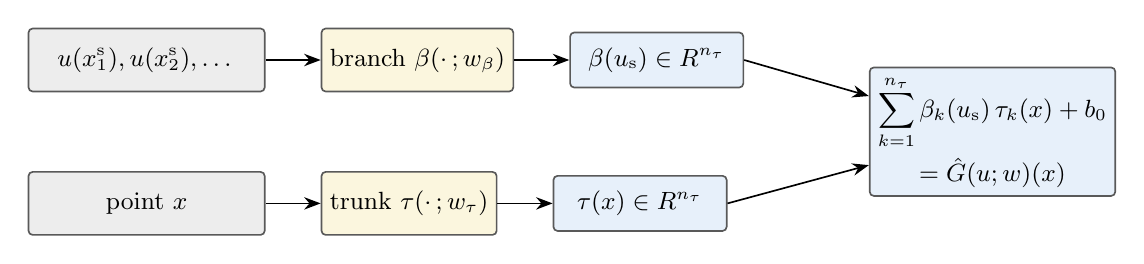
\begin{tikzpicture}[every node/.append style={font=\small}, node distance=6mm and 7mm]
  \node[inputnode, minimum width=30mm] (u) {$u(x^{\mathrm s}_1),u(x^{\mathrm s}_2),\dots$};
  \node[opnode, right=of u, minimum width=22mm] (br) {branch $\bm\beta(\cdot\,;\W_\beta)$};
  \node[statenode, right=of br, minimum width=22mm] (be) {$\bm\beta(\bm u_{\mathrm s})\in\Real^{n_\tau}$};
  \node[inputnode, below=10mm of u, minimum width=30mm] (x) {point $x$};
  \node[opnode, right=of x, minimum width=22mm] (tr) {trunk $\bm\tau(\cdot\,;\W_\tau)$};
  \node[statenode, right=of tr, minimum width=22mm] (ta) {$\bm\tau(x)\in\Real^{n_\tau}$};
  \node[outputnode, right=28mm of $(be)!0.5!(ta)$, align=center]
    (out) {$\displaystyle\sum_{k=1}^{n_\tau}\beta_k(\bm u_{\mathrm s})\,\tau_k(x) + b_0$\\[2pt]$=\hat G(u;\W)(x)$};
  \draw[edge] (u) -- (br);
  \draw[edge] (br) -- (be);
  \draw[edge] (x) -- (tr);
  \draw[edge] (tr) -- (ta);
  \draw[edge] (be.east) -- (out);
  \draw[edge] (ta.east) -- (out);
\end{tikzpicture}
\end{document}
